\documentclass{article}
\usepackage[utf8]{inputenc}
\usepackage{graphicx}
\usepackage{subcaption}
\usepackage{float}
\usepackage{hyperref}
\usepackage{amsmath}
\newcommand{\mypapersize}{A4}
\title{Pattern Recognition Cheat Sheet}
\author{CCE 2020}
\begin{document}
\maketitle
\tableofcontents

%%%%%%%%%%%% Dimension Reduction Section %%%%%%%%%%%%%%%%%%%%
\section{Dimensionality Reduction}
    We reduce dimensionality to Compress Data, 
    Reduce Noise, Visualization and Apply Euclidean geometry comfortably.
    \subsection{PCA}
        \begin{itemize}
    \item Principal Component Analysis (PCA) is a dimension-reduction tool.
    \item The first principal component accounts for as much of the variability in the data as possible, and each succeeding component accounts for as much of the remaining variability as possible.
    \item PCA seeks a linear combination of variables such that the maximum variance is extracted from the variables.
    Those PCs are the eigenvectors decomposed and eigenvalues determine weight of each PC.
    \item \textbf{Explained Variance is ratio of eigenvalues. (PC eigenvalue / summation of all eigenvalues)}
    \begin{figure}[H]
        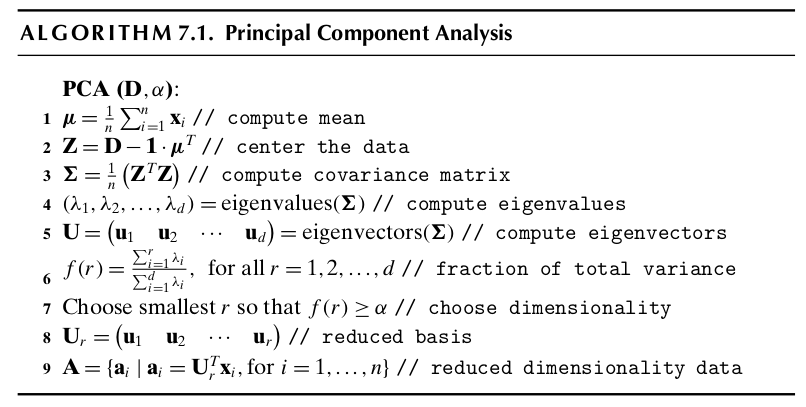
\includegraphics[width=\textwidth]{Figures/pca.png}
        \caption{\label{fig:figure1}PCA Algorithm}
    \end{figure}
\end{itemize}
    \subsection{LDA}
        \begin{itemize}
    \item The goal of linear discriminant analysis (LDA) is to find a vector w that maximizes the separation between the classes after projection onto w.
    \item The Fisher LDA objective: \[ \operatorname*{max}_w J(w) = \frac{(m_1 - m_2)^2}{s_1^2 + s_2^2}\] 
    \item We solve the problem by using the eigenvalue–eigenvector equation, as below. \[(S^{-1}B)w = \lambda w \]
    Thus, if \(S^{-1}\) exists, then \(\lambda\) = J(w) is an eigenvalue, and w is an eigenvector of the matrix
    \(S^{-1}\) B. To maximize J(w) we look for the largest eigenvalue \(\lambda\), and the corresponding dominant eigenvector w specifies the best linear discriminant vector.
    \item The key difference between principal component analysis and LDA is that the former deals with unlabeled data and tries to maximize variance, whereas the latter deals with labeled data and tries to maximize the discrimination between the classes.
    \begin{figure}[H]
        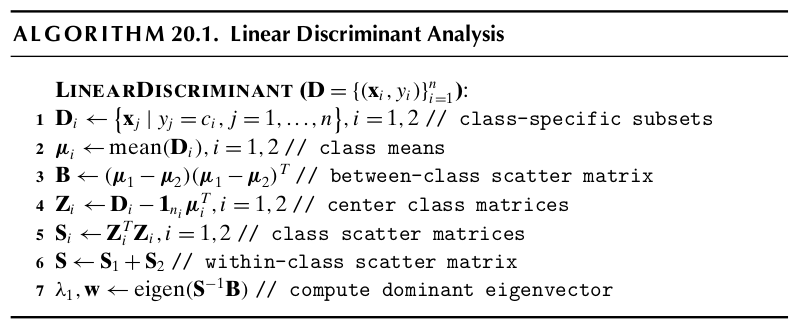
\includegraphics[width=\textwidth]{Figures/lda.png}
        \caption{\label{fig:figure2}LDA Algorithm, total time is
        O($d^3$ + $nd^2$).}
    \end{figure}
\end{itemize}

%%%%%%%%%%%% Clustering Section %%%%%%%%%%%%%%%%%%%%
\section{Unsupervised Learning: Clustering}
    \subsection{K-means Clustering}
        \begin{itemize}
    \item K-means  uses Euclidean Distance, uses Mean as representative: Centroid
    \item K-means  has a parameter K that you need to guess before clustering (Choice of K is crucial, may stuck at local minimum)
    \item \textbf{Failure in case of non spherical data but FAST !}
    \item Iterative two-step approach?  1- Cluster Assignment,  2- Centroid Update\\When to stop?  1- No update in the assignment  , 2- Max iterations reached
    \item \textbf{Randomness of K-means}: Centroids are chosen first at random , May not find the same solution every time. Then, run several times, and the run with the lowest SSE value is chosen to report the final clustering.
    \begin{figure}[H]
        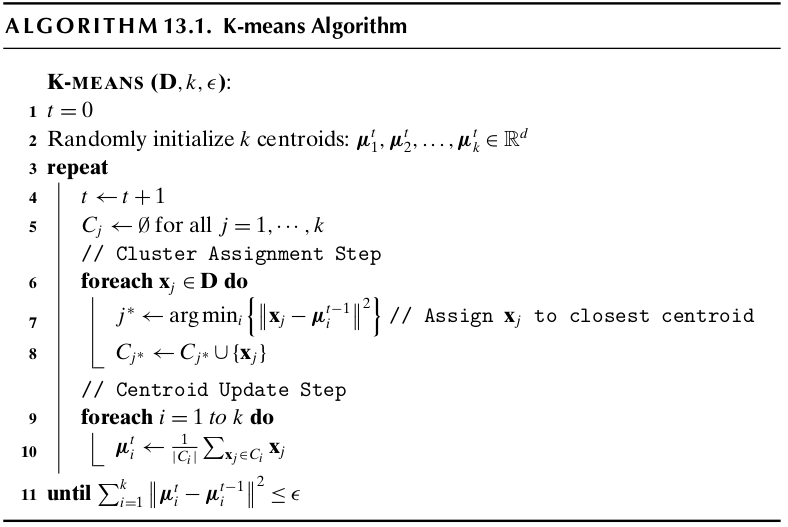
\includegraphics[width=0.8\textwidth]{Figures/kmeans.png}
        \caption{\label{fig:figure3}K-Means Algorithm, total time is O(tknd).}
    \end{figure}
\end{itemize}
    \subsection{Spectral Clustering }
        \begin{itemize}
    \item Consider clustering over graph data, that is, given a graph, the goal is to cluster the nodes by using the edges and their weights, which represent the similarity between the incident nodes.
    \item Similarity is a relative quantity between two instances, High when similar and Low when dissimilar.\textbf{Distance is a dissimilarity measure.}
    \item For n data instances,We have ($n^2$) similarities to be computed and pack them into a similarity matrix (A) where it can be viewed as weighted adjacency matrix of a graph.
    \begin{figure}[H]
        \centerline{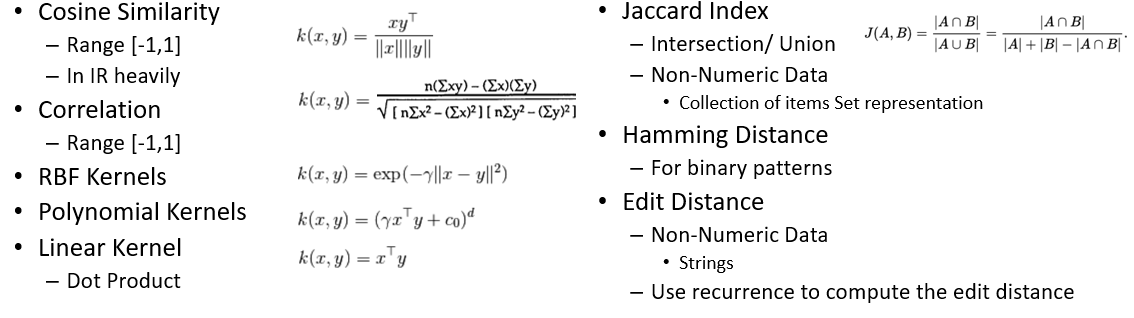
\includegraphics[width=1.5\textwidth]{Figures/sim.png}}
        \caption{\label{fig:figure5}Similarity Measures}
    \end{figure}
    \item In graph theory, a minimum cut of a graph is a cut that partition graph into two sets A and B such that weight of edges connecting vertices in A to vertices in B is minimum.
    \item Easy to solve O(VE) algorithm But Not satisfactory partition as it tends often to isolate vertices
    \begin{figure}[H]
        \centerline{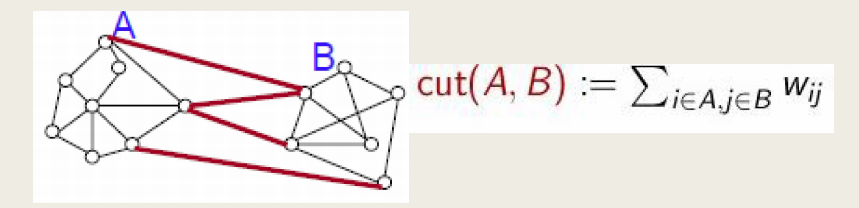
\includegraphics[width=\textwidth]{Figures/mincut.png}}
        \caption{\label{fig:figure6}Minimum Cut Rule}
    \end{figure}
    \item Normalized cut however works to partition graph into two sets A and B such that weight of edges connecting vertices in A to vertices in B is minimum and size of A and B are very similar.
    \item However, the main problem we face is that the eigenvectors u i are not binary, and thus
    it is not immediately clear how we can assign points to clusters. One solution to this
    problem is to treat the n x k matrix of eigenvectors as a new data matrix.
    \begin{figure}[H]
        \centerline{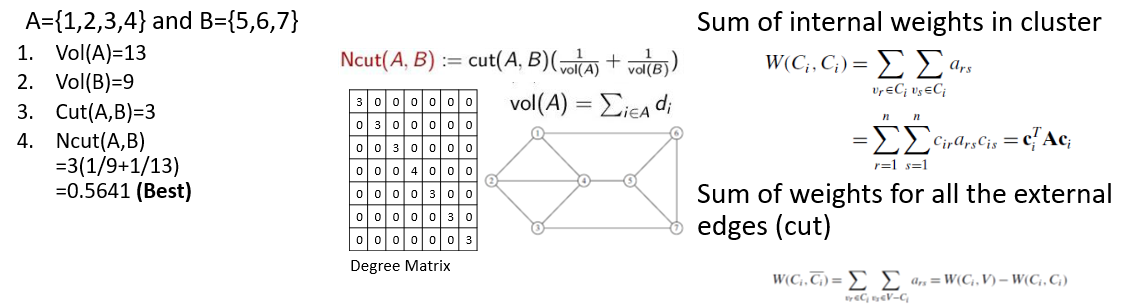
\includegraphics[width=1.6\textwidth]{Figures/normcut.png}}
        \caption{\label{fig:figure7}Normalized Cut}
    \end{figure}
    \begin{figure}[H]
        \centerline{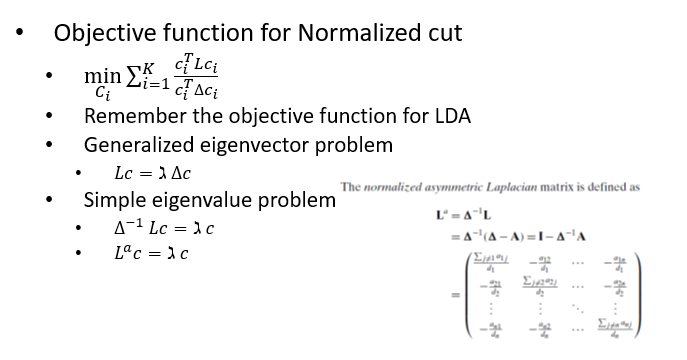
\includegraphics[width=1.4\textwidth]{Figures/spectral2.png}}
        \caption{\label{fig:figure8}Spectral Clustering Objective Function}
    \end{figure}
    \begin{figure}[H]
        \centerline{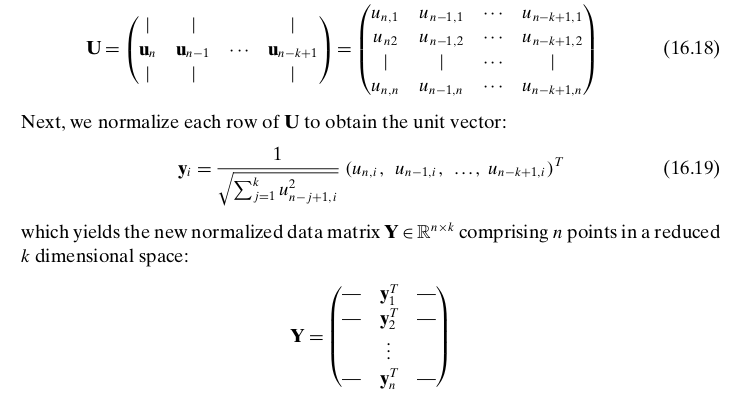
\includegraphics[width=1.2\textwidth]{Figures/yspectral.png}}
        \caption{\label{fig:figure9}Normalized Eigenvectors}
    \end{figure}
    \item \textbf{Applying k-means to Laplacian eigenvectors allows us to find cluster with non-convex boundaries.}
    \item Some Issues are the choice of number of clusters k, choice of similarity measure, for RBF Gaussian kernels, choice of $\gamma$.
    \item Complexity is as follows, Construction of the similarity matrix O($n^2$d)and Eigenvalue decomposition O($n^3$)
    \begin{figure}[H]
        \centerline{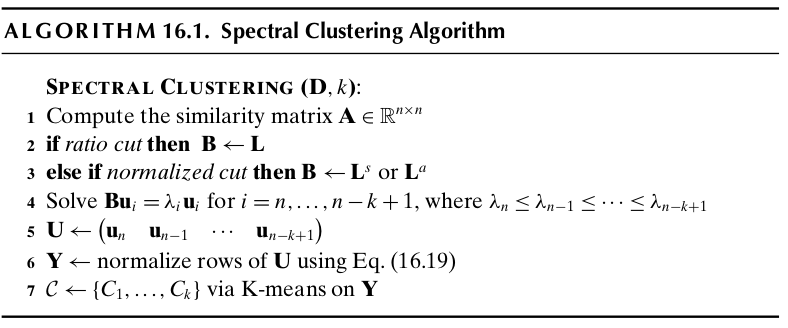
\includegraphics[width=\textwidth]{Figures/spectral.png}}
        \caption{\label{fig:figure10}Normalized Cut Algorithm}
    \end{figure}
\end{itemize}
    \subsection{Clustering Evaluation}
        \begin{itemize}
    \item External: External validation measures employ criteria that are not inherent to the dataset. This can be in form of prior or expert-specified knowledge about the clusters, for example, class labels for each point.
    \item Internal: Internal validation measures employ criteria that are derived from the data
    itself. For instance, we can use intracluster and intercluster distances to obtain measures of cluster compactness (e.g., how similar are the points in the same cluster?) and separation (e.g., how far apart are the points in different clusters?).
    \item Purity: When r = k, a purity value of 1
    indicates a perfect clustering, with a one-to-one correspondence between the clusters
    and partitions. However, purity can be 1 even for $r > k$, when each of the clusters is a
    subset of a ground-truth partition. When $r < k$, purity can never be 1, because at least one cluster must contain points from more than one partition.
    \item F-measure: the higher this value the better, this is better than purity in that the value of the recall measures how representative the cluster is of the partition it represents.For a perfect clustering, when r = k, the maximum value of the F-measure is 1.
    \begin{figure}[H]
        \centerline{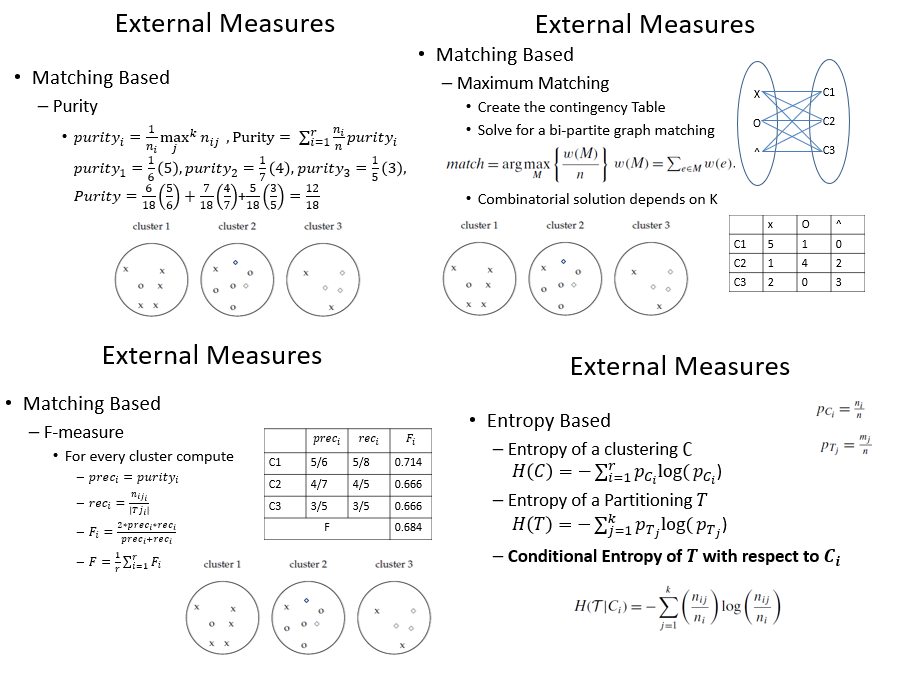
\includegraphics[width=1.5\textwidth]{Figures/externalmes.png}}
        \caption{\label{fig:figure11}External Measures}
    \end{figure}
    \item Conditional Entropy: measures how the clustering reduced the entropy of the ground truth,min value=0, max value = entropy of ground truth. The lower the value of this the better. For a perfect clustering, the conditional entropy value is zero, whereas the worst possible conditional entropy value is log k.
    \item For Jaccard and Rand indices, the larger the better. A prefect clustering has a value of 1 for both, Jaccard Index favors a clustering that puts points from the same ground truth partition together disregarding points not in the same ground truth partition appearing together.
    \begin{figure}[H]
        \centerline{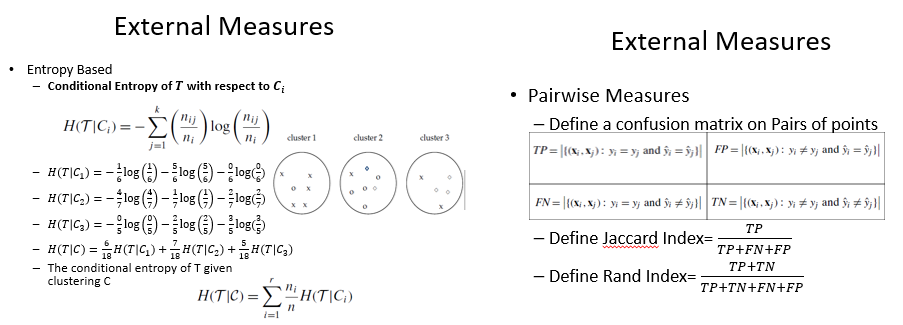
\includegraphics[width=1.5\textwidth]{Figures/externalmes2.png}}
        \caption{\label{fig:figure12}External Measures: Continue}
    \end{figure}
    \begin{figure}[H]
        \centerline{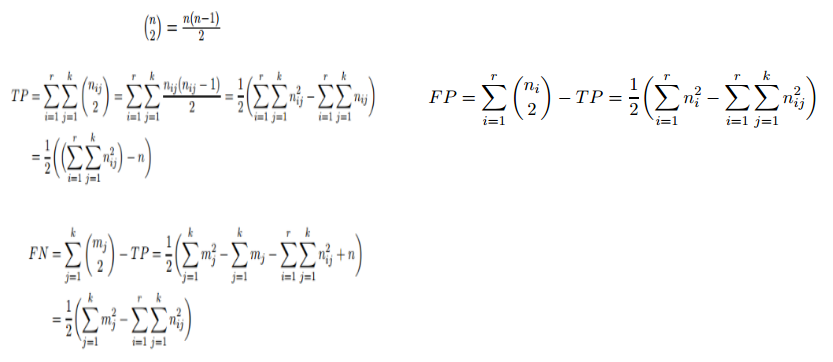
\includegraphics[width=1.5\textwidth]{Figures/externalmes3.png}}
        \caption{\label{fig:figure13}External Measures: Continue}
    \end{figure}
    $$TN = N- (TP + FP + FN)$$
    \[ purity(D_j) = \operatorname*{max}_i {\frac{n_{ij}}{n_j}}\] 
    \newpage
    \item Internal Measures treat with Clustering C as cut in a proximity (distance) matrix. The Graph(V,E) has V points and E edges. Edge weight is the proximity between two points. Given any subsets S,R (subset from V), define W(S,R) as the sum of the weights on all edges with one vertex in S and the other in R, given as
    \begin{figure}[H]
        \centerline{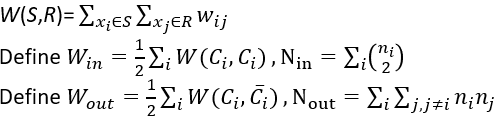
\includegraphics[width=0.8\textwidth]{Figures/internalmes.png}}
        \caption{\label{fig:figure14}Rules to get internal Measures}
    \end{figure}
    \begin{figure}[H]
        \centerline{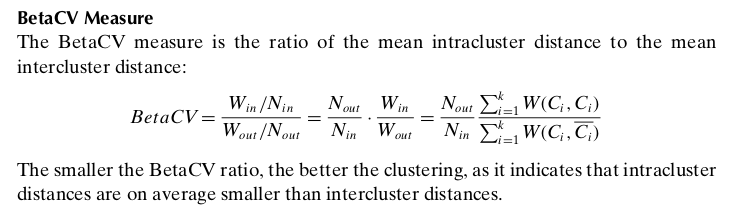
\includegraphics[width=1.1\textwidth]{Figures/beta.png}}
        \caption{\label{fig:figure15}Beta CV Measure}
    \end{figure}
    \begin{figure}[H]
        \centerline{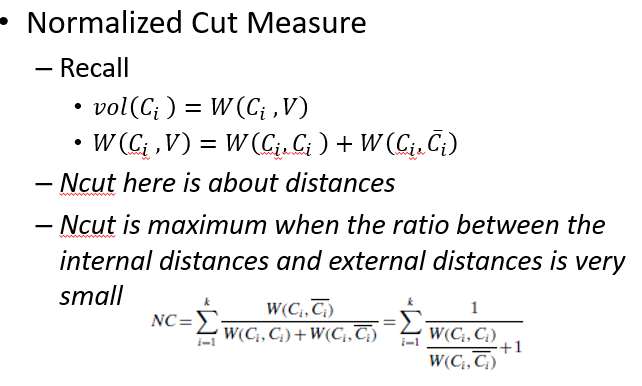
\includegraphics[width=0.9\textwidth]{Figures/internalmes2.png}}
        \caption{\label{fig:figure16}Normalized Cut measure}
    \end{figure}
    \begin{figure}[H]
        \caption{\label{fig:figure}Internal Measures Example}
        \centerline{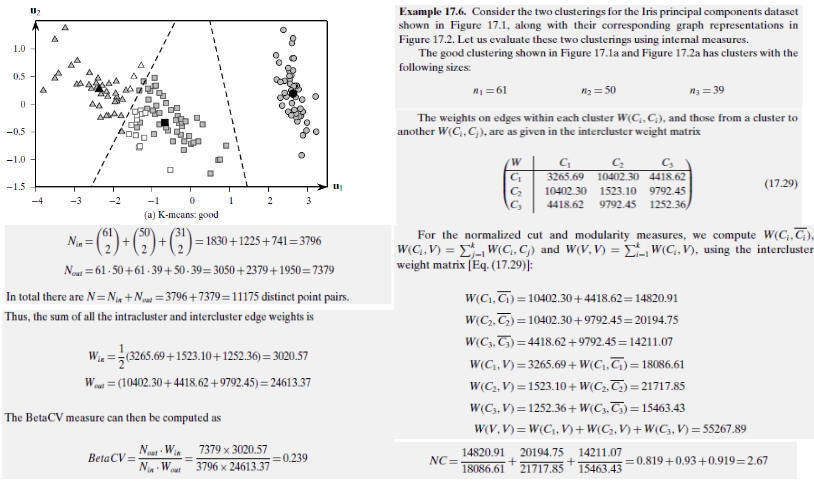
\includegraphics[width=1.5\textwidth]{Figures/cluster}}
    \end{figure}
    \item Beta-CV: The lower the better, measures the ratio internal cluster weights to cluster separation distance.This indicates that intracluster distances are on average smaller than intercluster distances.
    \item Normalized cut: The higher the value of this, the better it is, this is because we use a distance matrix and not a similarity matrix. The maximum possible value of NC is k.
\end{itemize}
    \newpage

%%%%%%%%%%%% Classification Section %%%%%%%%%%%%
\section{Supervised Learning: Classification}
    Classification Pipeline includes: Input (training set), Learning a model and Evaluation of the quality of the classifier by asking it to predict labels for a new set of objects that it
    has never seen before (test set) then compare the true labels of these objects to the ones predicted by the classifier.
    \subsection{KNN: K- Nearest Neighbour Classifier}
        \begin{itemize}
\item A non-parametric approach, which does
not make any assumptions about the underlying joint probability density function.Instead, it directly uses the data sample to estimate the density. Therefore, KNN could and probably should be one of the first choices for a classification study when there is little or no prior knowledge about the distribution data.
\item KNN is also a lazy algorithm .No Training ! Lack of generalization means that KNN keeps all the training data. To be more exact, all (or most) the training data is needed during the testing phase.
\item So, the predicted class for point x equation is given below where Ki is the neighbours of x.
\begin{figure}[H]
\centerline{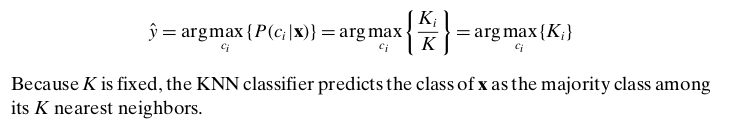
\includegraphics[width=1.2\textwidth]{Figures/knn.png}}
\caption{\label{fig:figure17}KNN Predicted Class Equation}
\end{figure}
\item KNN needs parameter tuning on the K which is the number of neighbors used to vote for the label and the distance function used to find the closest sample(s).
\item NEVER use the test set for the purpose of tweaking hyper parameters.\\For measuring the generalization of your classifier, Use the test set once at end.Use Validation sets for Hyper parameter Tuning.
\item Cross Validation for Classifier Tuning: 5-fold cross-validation run for the parameter k. For each value of k we train on 4 folds and evaluate on the 5th. For each k we receive 5 accuracies on the validation fold.\\
If we used more than 5 folds, we might expect to see a smoother (i.e. less noisy) curve.
\end{itemize}
    \subsection{Full Bayes Classifier}
        \begin{itemize}
    \item The Bayes classifier directly uses the Bayes theorem to predict the class for a new test instance, x. It estimates the posterior probability $P (c_i|x)$ for each class $c_i$ , and chooses the class that has the largest probability. The predicted class for x is given as
    \[ y = \operatorname*{argmax}_{c_i} P (c_i|x)\]
    \[ P (c_i|x) = \frac{P(x|c_i)P(c_i)}{P(x)}\]
    or for ease we can discard P(x).
    \item Estimate Prior Probability: $P(c_i) = \frac{n_i}{n}$
    \item Estimate probability of observing x from any of the k classes: $$P(x) = \sum_{j=1}^k{P(x|c_j)P(j)}$$
    \item Estimate Likelihood of Numeric attribute:
\begin{figure}[H]
\centerline{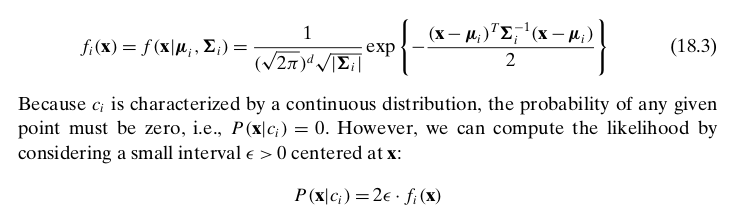
\includegraphics[width=1.3\textwidth]{Figures/bayes1.png}}
\end{figure}
    \item Estimate Likelihood of Categorical attribute:
\begin{figure}[H]
\centerline{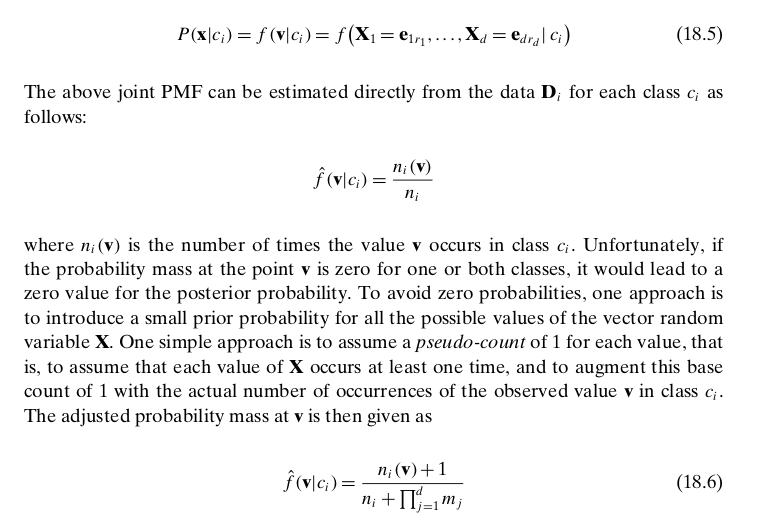
\includegraphics[width=1.1\textwidth]{Figures/bayes2.png}}
\end{figure}  
\begin{figure}[H]
\centerline{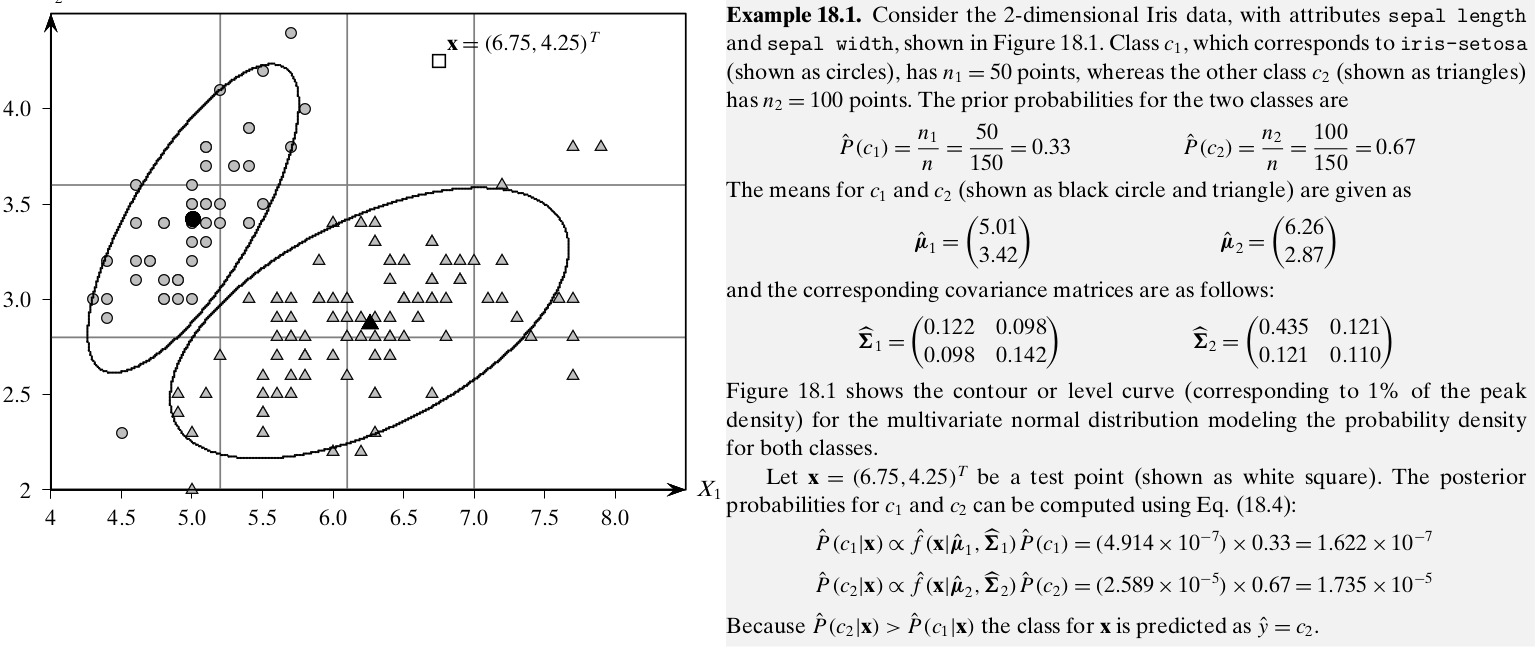
\includegraphics[width=1.3\textwidth]{Figures/bayes_ex}}
\end{figure}
    \item Classes are parameterized with mean vector and covariance matrix.This might not hold true for all cases.Too many parameters to be estimated. (For numeric attributes, $O(d^2)$ covariances).  Use Naive !
\begin{figure}[H]
\centerline{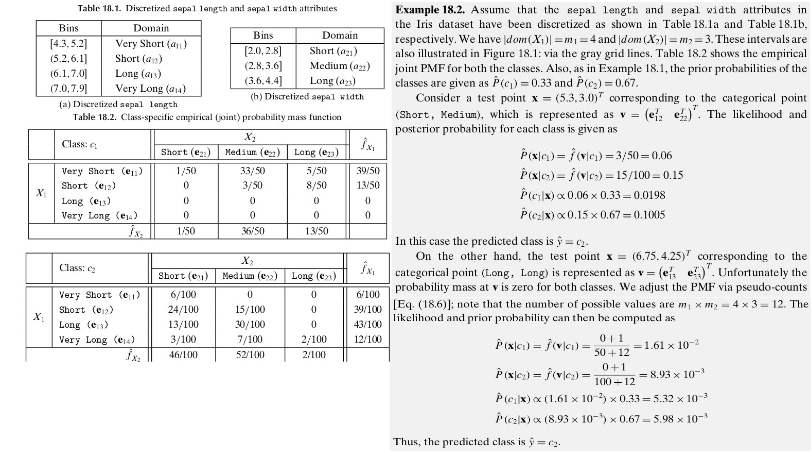
\includegraphics[width=1.2\textwidth]{Figures/bayes3}}
\end{figure}
    
\end{itemize}
    \subsection{Naive Bayes Classifier}
        \begin{itemize}
 \item The naive Bayes approach makes the simple assumption that all the attributes are independent. This leads to a much simpler, though surprisingly effective classifier in practice.
 \item The naive Bayes classifier uses the sample mean and a diagonal sample covariance matrix for each class $c_i$ . Thus, in total 2d parameters have to be estimated, corresponding to the sample mean and sample variance for each dimension $X_j$ .
\begin{figure}[H]
\centerline{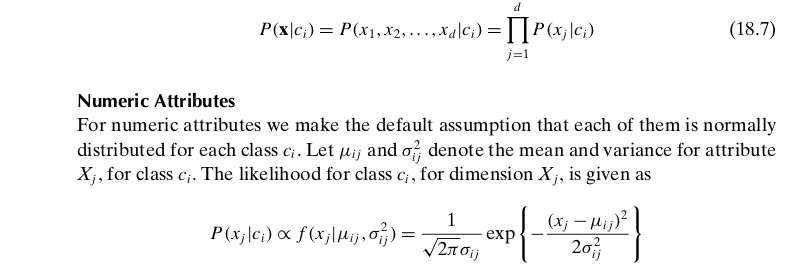
\includegraphics[width=1.2\textwidth]{Figures/naive}}
\caption{\label{fig:figure21}Likelihood Estimation in Naive Bayes ,Numeric}
\end{figure}
\begin{figure}[H]
\centerline{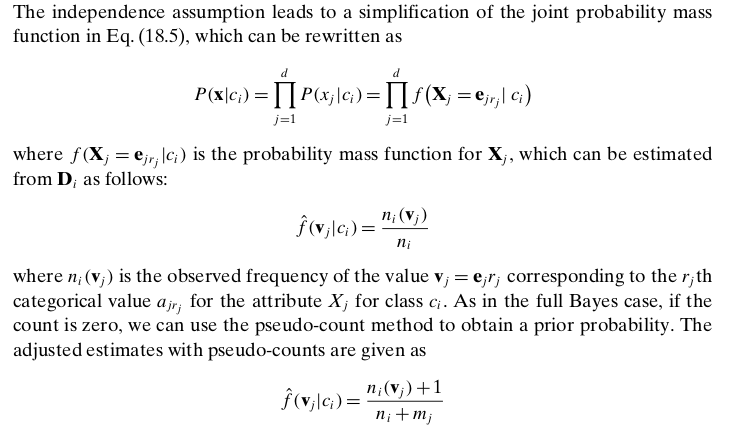
\includegraphics[width=1.1\textwidth]{Figures/naive2}}
\caption{\label{fig:figure22}Likelihood Estimation in Naive Bayes ,Categorical}
\end{figure}
\begin{figure}[H]
\centerline{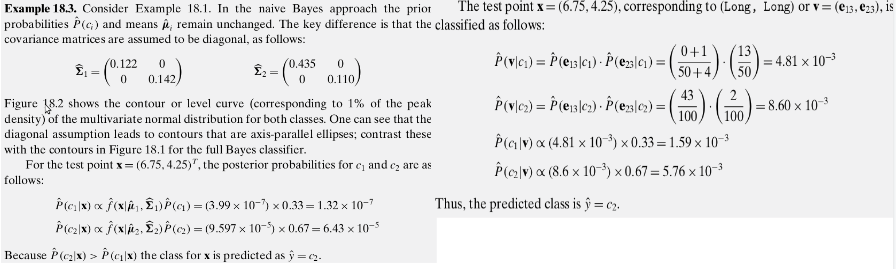
\includegraphics[width=1.7\textwidth]{Figures/bayes4}}
\end{figure}
\end{itemize}
    \newpage
    \subsection{Decision Tree Classifier}
        \begin{itemize}
    \item A decision tree classifier is a recursive partition-based tree model that predicts the class $y_i$ for each point $x_i$.
    \item A decision tree uses axis-parallel hyperplanes.
    \item To classify a new test point we have to recursively evaluate which half-space it belongs to until we reach a leaf node in the decision tree, at which point we predict its class as the label of the leaf.
    \item Advantages include easily interpretable models, supports multi-class and handles both numeric and categoric data. Disadvantages is it can cause over fitting if used bad threshold values for input.
    \begin{figure}[H]
        \centerline{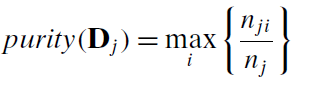
\includegraphics[width=0.4\textwidth]{Figures/dt1}}
        \caption{\label{fig:figure}Purity Rule}
    \end{figure}
    \subsubsection{Split Point Measures: Information Gain}
        \begin{figure}[H]
            \centering
            \begin{minipage}{0.6\textwidth}
                \centering
                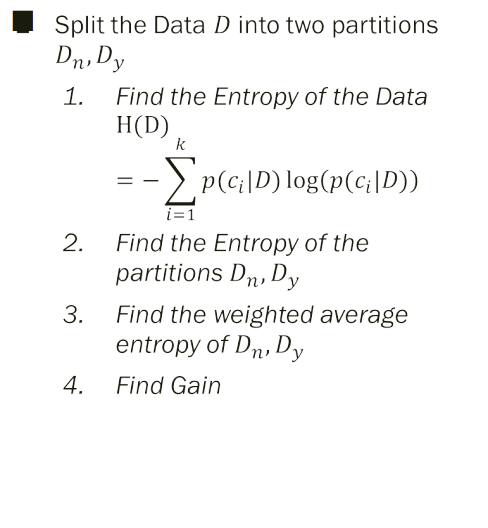
\includegraphics[width=0.9\textwidth]{Figures/dt2.png} % first figure itself
                \caption{Procedure}
            \end{minipage}\hfill
            \begin{minipage}{0.4\textwidth}
                \centering
                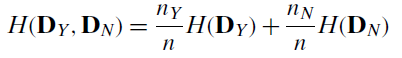
\includegraphics[width=\textwidth]{Figures/dt3.png} % second figure itself
                \caption{Split Entropy}
            \end{minipage}
            \begin{minipage}{0.4\textwidth}
                \centering
                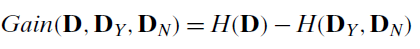
\includegraphics[width=\textwidth]{Figures/dt4.png} % second figure itself
                \caption{Gain}
            \end{minipage}
        \end{figure}
        \textbf{The Higher the better}
    \subsubsection{Split Point Measures: Gini-Index}    
\begin{figure}[H]
    \centering
    \begin{minipage}{0.5\textwidth}
        \centering
        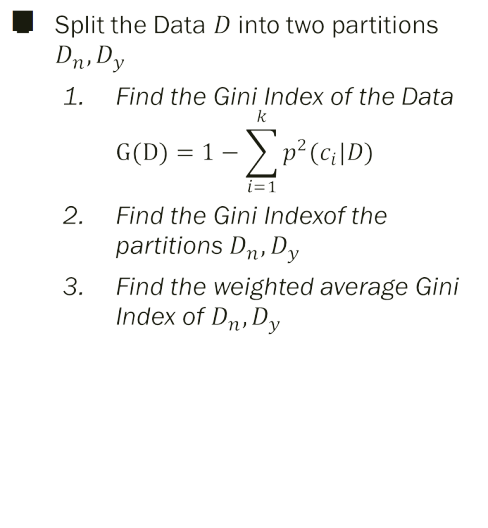
\includegraphics[width=\textwidth]{Figures/dt5.png} % first figure itself
        \caption{Procedure}
    \end{minipage}\hfill
    \begin{minipage}{0.5\textwidth}
        \centering
        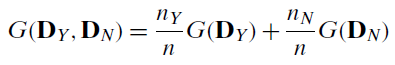
\includegraphics[width=\textwidth]{Figures/dt6.png} % second figure itself
        \caption{Weighted Gini-Index for Split Point}
    \end{minipage}
\end{figure}
\textbf{The Lower the better}
\textbf{The Gini coefficient provides an index to measure impurity}
\begin{figure}[H]
\centerline{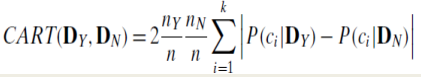
\includegraphics[width=0.7\textwidth]{Figures/cart}}
\caption{\label{fig:figure}Cart Measure Rule}
\end{figure}

    \item For a numeric attribute x, How to find the split value?Use midpoint of the possible distinct values for x because it is bounded by the number of distinct points which is at most all points. 
\end{itemize}

\subsubsection{Numeric Example}
\begin{figure}[H]
\centerline{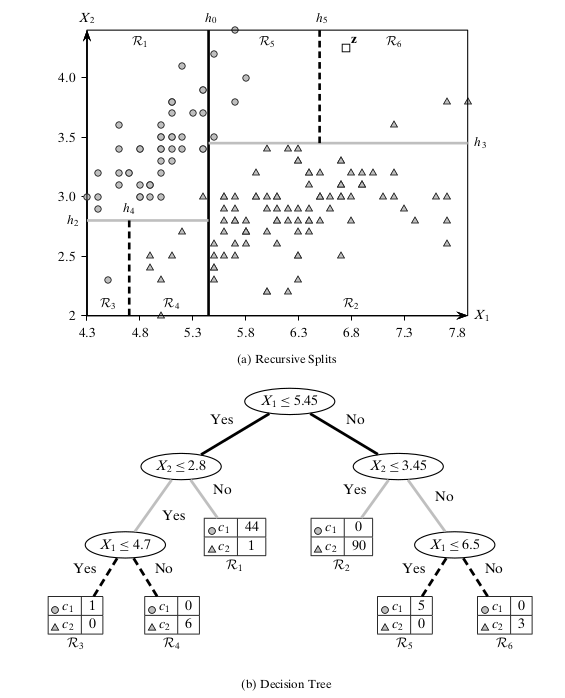
\includegraphics[width=\textwidth]{Figures/dt8}}
\caption{\label{fig:figure}Data and Generated Tree}
\end{figure}
\begin{figure}[H]
\centerline{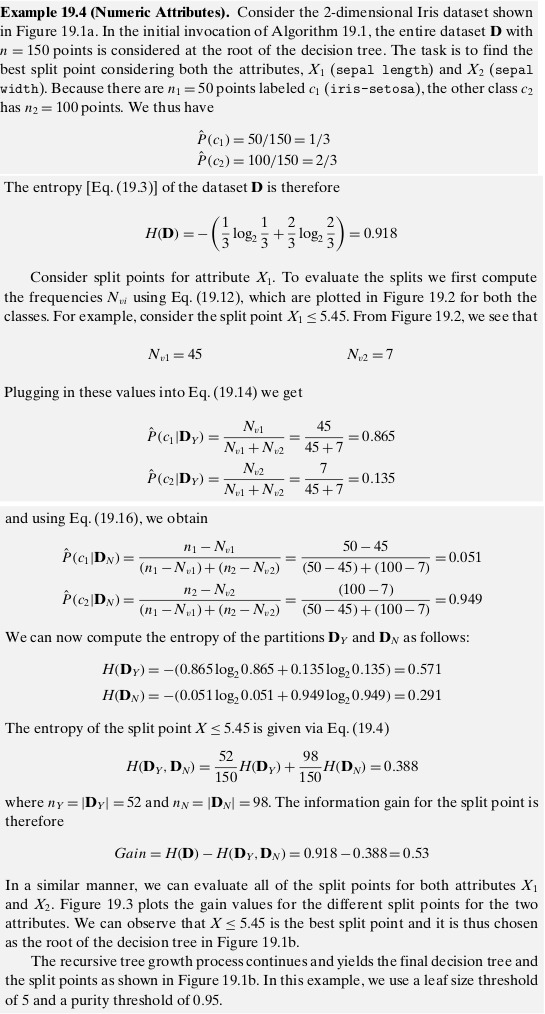
\includegraphics[width=\textwidth]{Figures/dt11}}
\caption{\label{fig:figure}Solution for Numeric Attributes}
\end{figure}
\begin{figure}[H]
\centerline{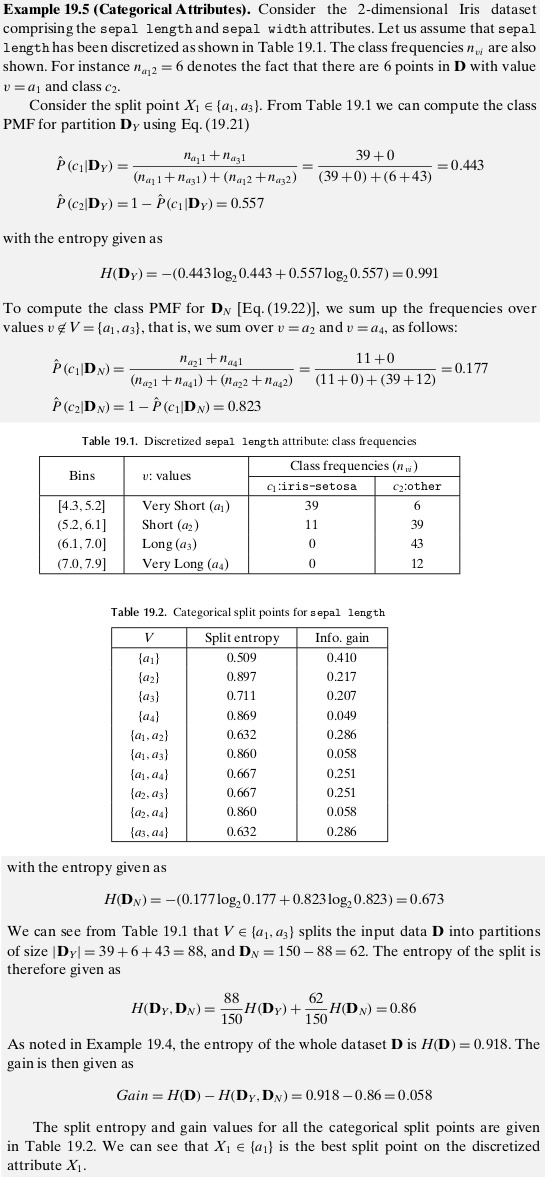
\includegraphics[width=0.9\textwidth]{Figures/dt12}}
\caption{\label{fig:figure}Solution for Categorical Attributes}
\end{figure}
    \newpage
    \subsection{Ensemble Methods}
        \begin{itemize}
    \item The idea is to combine the results of multiple classifiers for the same problem.
    \item \textbf{Bias} is the systematic deviation of its predicted decision boundary from the true decision boundary
    \item \textbf{Variance} is the deviation among the learned decision boundaries over different training sets.
    \item \textbf{Unstable classifier} is when small perturbations in the training set will result in large changes in the prediction. They have High variance and are subject to Overfitting.
    \item \textbf{Less complex classifiers} underfit the data, and usually have low variance, high bias.
    \item So we use Base Classifiers: trained on different subsets of data and produce Combined Classifier. With the Objective is to reduce bias and variance where we model complex classifiers using many simple ones.
    
\begin{figure}[H]
\centerline{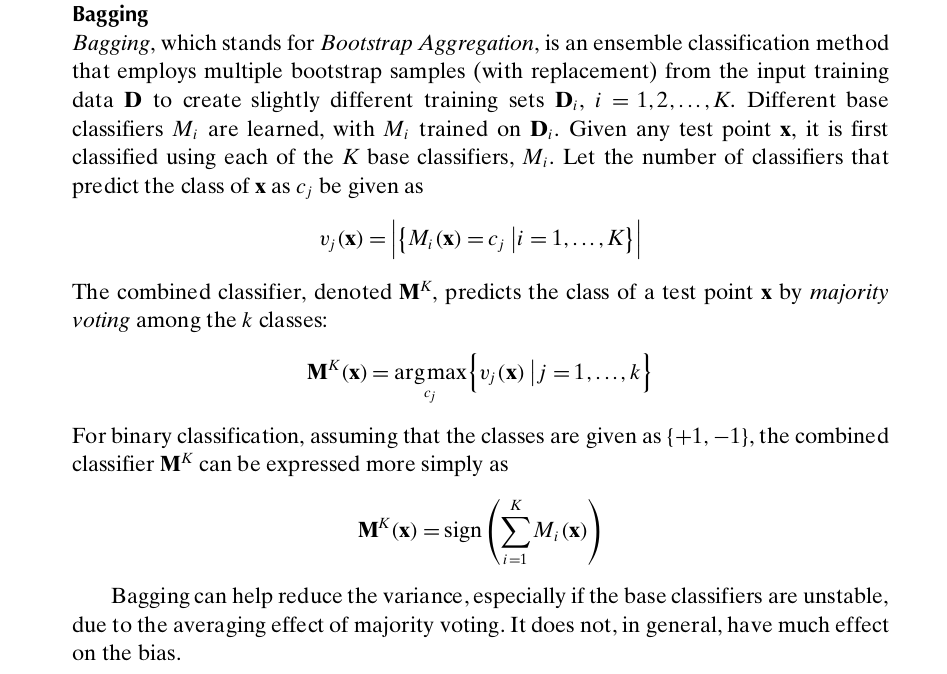
\includegraphics[width=1.2\textwidth]{Figures/bagging}}
\caption{\label{fig:figure}Bagging Method}
\end{figure}
\begin{figure}[H]
\centerline{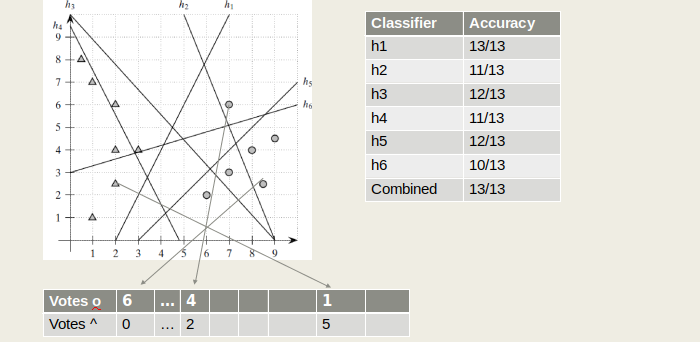
\includegraphics[width=\textwidth]{Figures/bagging2}}
\caption{\label{fig:figure}Example on Bagging Method}
\end{figure}


\begin{figure}[H]
    \centering
    \begin{minipage}{0.9\textwidth}
        \centering
        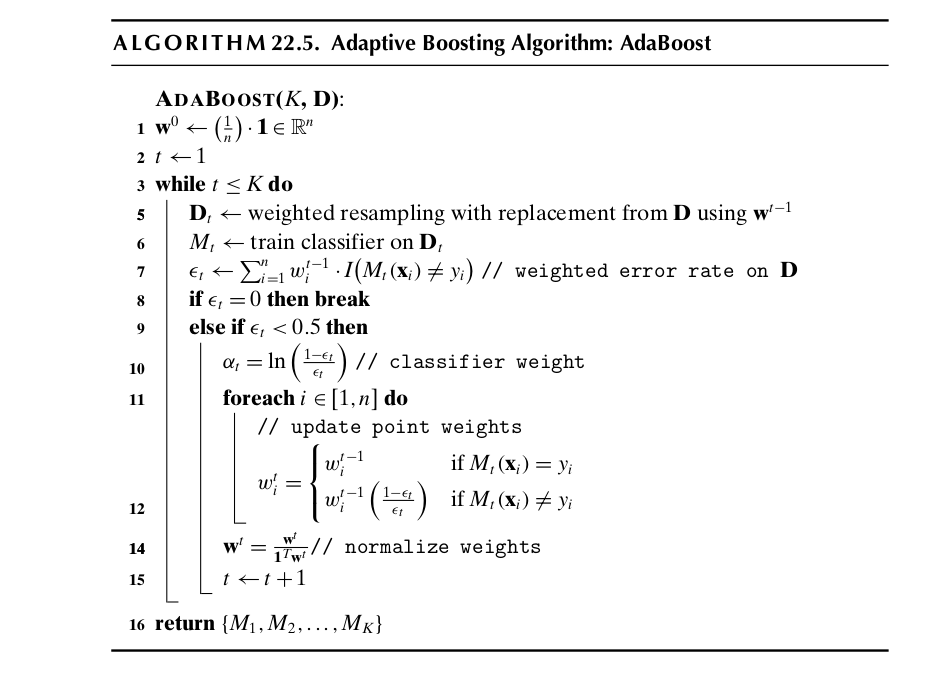
\includegraphics[width=\textwidth]{Figures/adaboost.png} % first figure itself
        \caption{Procedure}
    \end{minipage}\hfill
    \begin{minipage}{0.4\textwidth}
        \centering
        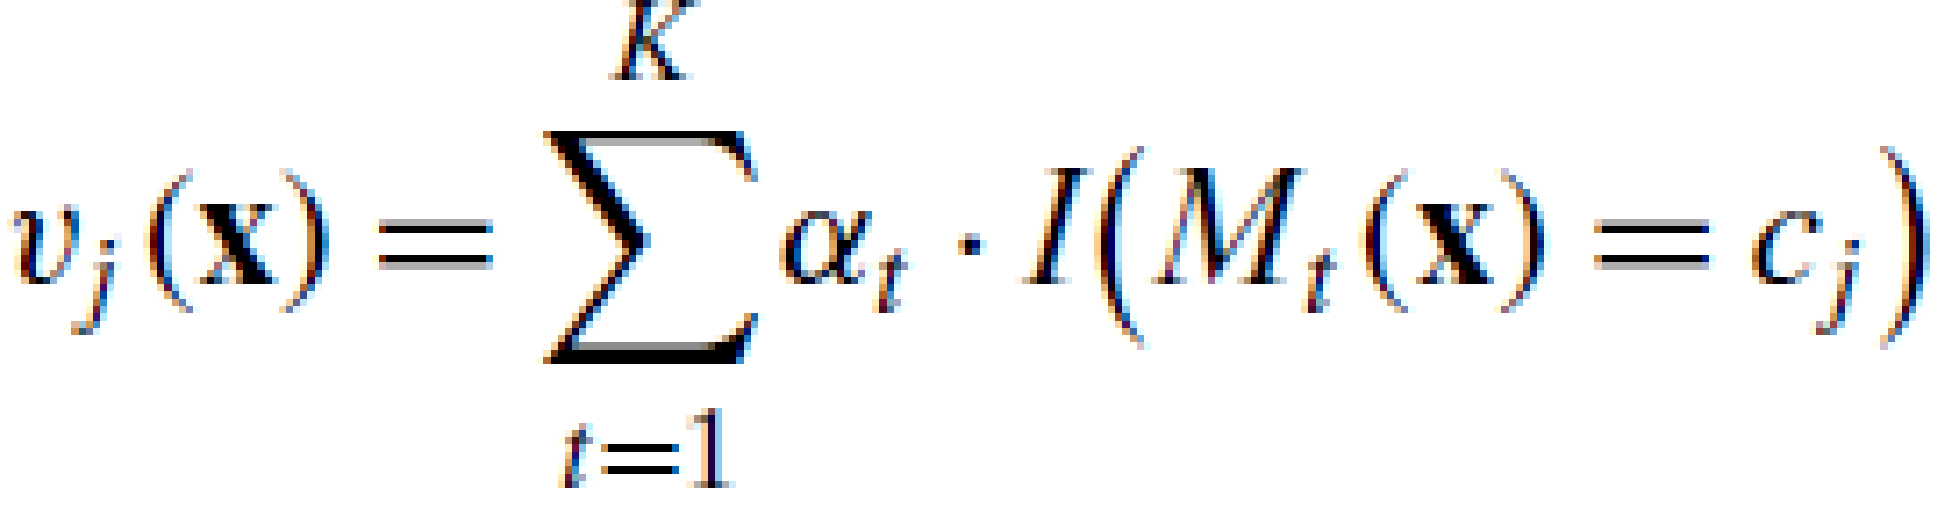
\includegraphics[width=\textwidth]{Figures/adaboost3.png} % second figure itself
    \end{minipage}
        \begin{minipage}{0.4\textwidth}
        \centering
        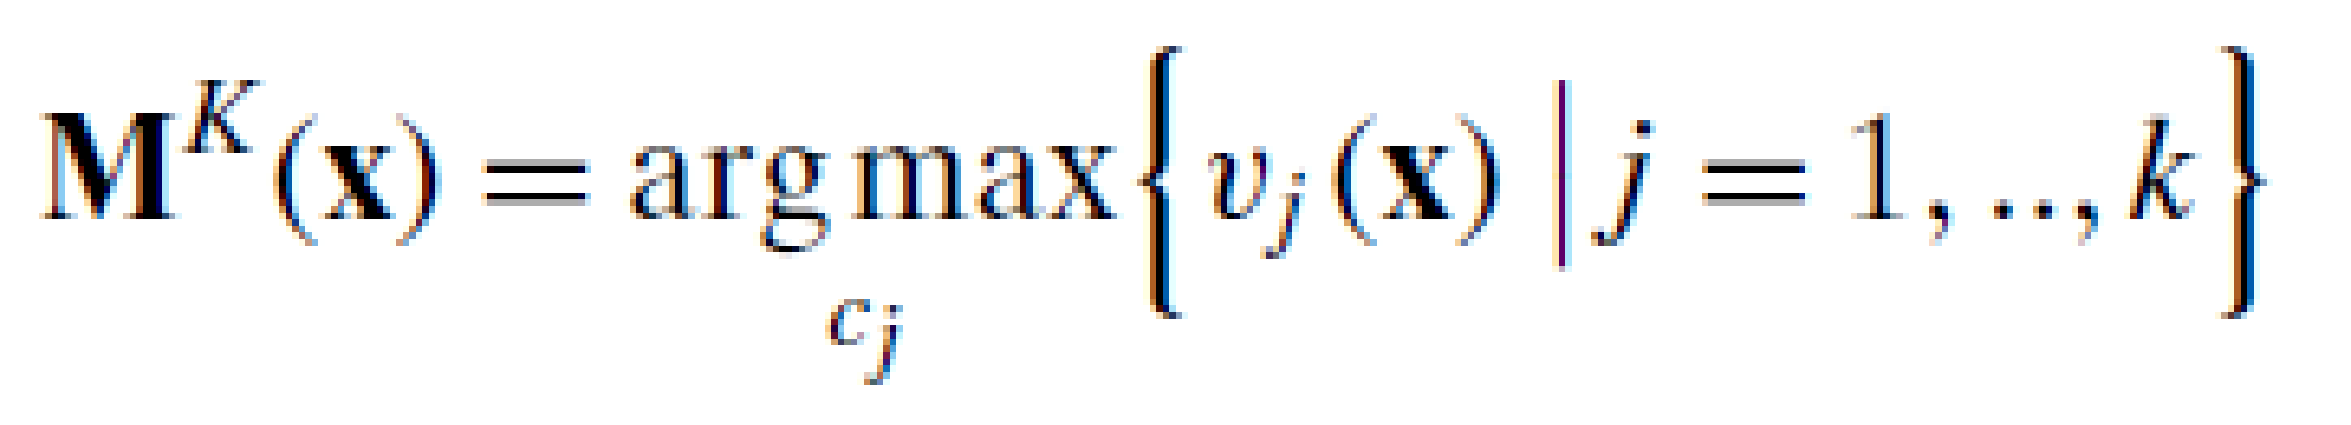
\includegraphics[width=\textwidth]{Figures/adaboost4.png} % second figure itself
    \end{minipage}
\end{figure}
\begin{figure}[H]
\centerline{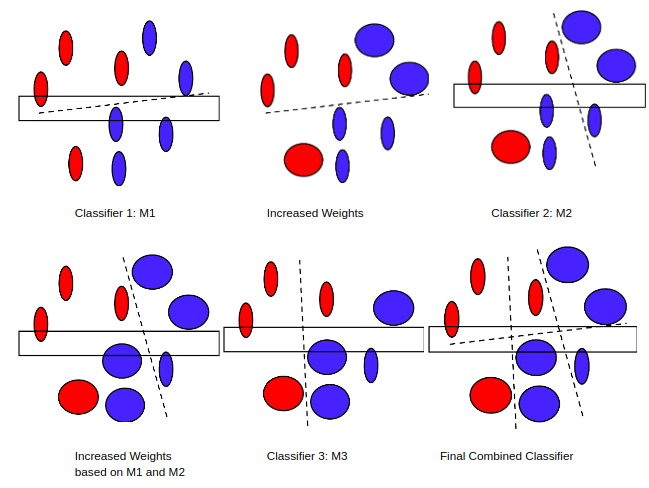
\includegraphics[width=1.2\textwidth]{Figures/adaboost2}}
\caption{\label{fig:figure}Example on Adaboost Method}
\end{figure}
    \item AdaBoost Notes
    \begin{itemize}
        \item Multiclass support? Yes. It can work for multi-class classification	
        \item Causes Reduction of variance due to averaging and Reduction of bias due to selecting harder examples
        \item Bagging is a special case of adaboost with Equal prob. of samples and Equal prob. of classifiers weights. It Reduces variance due to averaging.
        \item Supports non-linearity.
        \item May overfit the data.
    \end{itemize}




\end{itemize}

